\documentclass{report}
\usepackage{notes}

\begin{document}
\section{Preface}
All the content herein are from \href{https://youtu.be/V-DKcohQEvg}{lectures} given by Professor Ali Hajimiri. If you have the time, I would highly recommend watching the lectures as Professor Hajimiri is a great teacher who always goes back to first principles in his explanations where possible, and instills a great deal of clarity of the foundations. \smallskip \\
Due to the lack to information on the web about the Heaviside Operator, I've typed up these notes from his lectures. All examples herein are from the lectures, and one can refer to them if the calculations don't make sense. \smallskip \\
Please feel free to use these notes and the latex however you see fit. I hope you find this material as useful as I did. 

% \\
% \\
% Operator Domain
% [Heaviside] Operator Method gets operator for function in time domain consists of: replacing all d/dx with p, simplifying with partial fraction expansion
% p is the Heaviside Operator 
% converting between time and operator domain using a catalog
% \\
% \\
% Assumptions \\

\subsection*{Historical Aspect with Laplace Transform}
These notes \textbf{do not} assume you know Laplace Transform; however, the inquisitive reader who does know about the Laplace Transform will be wondering about how this method fits in with that. The notes do eventually go on to explain the Laplace Transform is a special case of the Operator Method, but till then, here is the interesting historical aspect from \href{https://youtu.be/V-DKcohQEvg}{Professor Hajimiri} to satisfy your curiosity: \smallskip \\
"... Oliver Heaviside was a very interesting character. He was engineer really, but he developed all these mathematical techniques, and he was the one who applied this operator method to solving [differential] equations, and to solving circuit problems and so on. But he was not a classic mathematician in the sense that he wouldn't prove things, he wouldn't think that it was necessary to prove things. So what happened is that he got into these fights with people who were in the business of proving things, sometimes useless things, but nonetheless they were in that business. So he got into fights with these people and eventually some of these people said, "Okay, wait a second. It seems that this is working so they went and tried to prove it and the way they proved the background of these things was using complex contours, complex calculations, complex integrals and improper integrals, and eventually what it turned out that it is was some variation of something that Laplace had done at some point in their life and they called it Laplace Transform. Now, Laplace Transform is a lot less general than the Heaviside approach because it relies on improper integrals, and convergence of improper integrals. But because everyone hated Oliver Heaviside, everyone switched to Laplace Transform. They couldn't bring themselves to use his method, although it was a very good method. So the lesson in that is that if you come up with good methods, it is also helpful to be nice to people."


\section{1. Overview}
\subsection*{Where are we now? Where have we been?}
Since these notes don't start form the beginning (i.e. from Observations of Nature and Maxwell's Equations), this section clarifies what we assume the reader to be familiar with.

\begin{center}
  \makebox[\textwidth]{\includegraphics[width=350]{overview.png}}
  \caption*{Overview of the field of EECS. 
  Anant Agarwal and Jeffrey Lang, course materials for 6.002 Circuits and Electronics, Spring 2007. MIT
OpenCourseWare (http://ocw.mit.edu/), Massachusetts Institute of Technology. Downloaded on [DD Month YYYY]}
\end{center}

We start by collection data about what we observe in nature through controlled experiments. These controlled experiments lead to tables of data from which we create abstractions that we call "Physical Laws", such as Maxwell's Equations. Maxwell's Equations give us a \textbf{mathematical model} [It's important to distinguish between mathematical and physical models. Two mathematically/electrically equivalent systems aren't physically equivalent. 
For example, if you take a circuit and put its Thevenin equivalent circuit in a black box and its Norton equivalent circuit in another black box, how would you know which is which? At their terminals, any external circuit would experience the same voltage and current from both boxes but the box with the Norton equivalent circuit would be warm, and would product a magnetic field as there is a current source present. This information is not captured by our mathematical model, and in this case we would need to update our model.] to understand how electric charges and electric current create electric and magnetic fields. These equations are however too unwieldy to use in general so we impose constrains on ourselves to play in a certain area of the playground of Electromagnetism. 

% [Disciplining ourselves to adhere to constrains to play in smaller areas of large playgrounds is a common theme in EECS that allows us make assumptions of how something will behave which simplify the models and equations we work with. The consequence of this is that we develop an attitude of not bothering about what happens outside these assumptions, which allows us to think in terms of logical relationships between the inputs and outputs to a system. 

% For example, this is the actual behavior of a resistor. 
% \begin{center}
%   \makebox[\textwidth]{\includegraphics[width=\textwidth]{resistor.png}}
%   \caption{Actual behavior of a resistor. https://youtu.be/hoO9Kb223rM?t=1331}
% \end{center}

% By disciplining ourselves to stay within a limited range of operation, we can simplify and characterise the behavior of a resistor using Ohm's Law. Further, these constrains ensure that constraints 2 and 3 of the Lumped Matter Discipline aren't broken. Thus, the initial set of constraints create additional constrains and the additional constrains ensure the initial constraints are adhered to - a self-reinforcing cycle. 

% This attitude is important as it allows us not to worry about "what if"s, and through generalising the logical relationships that stem from the assumptions, we can create powerful frameworks to understand systems (which is what these notes aim to explain).

% In practice, it may not always be possible to adhere to certain constrains, and in those cases, we either update the model of our elements (for example, two inductors in close proximity violate constraint 2 below and induce electric fields in another, in which case we can model the two inductors as a new element - a transformer), or add elements in our model (for example, parasitic capacitance/inductance can be included in our model by adding a capacitor/inductor).]

More specifically, the constrains we discipline ourselves to adhere to are [Agarwal and Lang, Chapter 1.3]:
\begin{enumerate}
    \item Dimensions of the circuit $<<$ The wavelength of light at the highest operating frequency of interest. 
    \item The boundaries of the discrete elements must be chosen so that
        $\pdv{\phi_{B}}{t} = 0$ through any closed path outside the element for all time.
    \item The elements must not include any net time-varying charge for all time. In other words, $\pdv{q}{t} = 0$, where q is the total charge within the element.
\end{enumerate}

To understand more about how these assumptions come about, and what their consequences are, Agarwal and Lang, Chapter 1.3 is a good resource.

As mentioned in the xxx first paragraph xxx, these constraints are assumptions we make about the Maxwell Equations that allow us to describe the voltage and currents across a set of elements in simple algebraic equations using Kirchhoff's Voltage Law, and Kirchhoff's Current Law. We then use these laws implicitly in Nodal Analysis, which can be used to solve any circuit. If we further discipline ourselves to operate such that all non-linear elements act linearly (constraining ourselves to operate in a narrow range around an operating point i.e. small signal/incremental method, for example), we can use Thevenin, Norton equivalent circuits, and Superposition to analyze circuits.\smallskip \\
The next step on our journey is to understand the relationship of current and voltage captured by resistors, capacitors and inductors. 

[Quick Recap
Capacitors -
At their basics, capacitors are elements whose charge depends on its voltage: $q(t) = C(t) x v(t)$ where C(t) is the capacitance of the capacitor at time t. We normally make the assumption that capacitance doesn't change with time, hence $q(t) = C x v(t)$. 
Since current is the flow of charge, $i = \dv{q}{t}$, and so the current of a capacitor is $i = \dv{q}{t} = C \dv{v}{t}$.

Inductors - At their basics, an element whose magnetic flux depends on current: $\phi = L(t) i$ where L is the inductance of the inductor at time t. Again, we usually make assumption that inductance is time-invariant so $\phi = L i$.
Now, voltage is the change in magnetic flux, $v(t) = \dv{\phi}{t} = L \dv{\phi}{t}$. Thus, $$i(t) = \frac{1}{L} \int_{-\infty}^{\infty} v(t) dt$$

In summary,
A resistor is an element whose current is proportion to its voltage.
A capacitor is an element whose current is proportional to the derivative of its voltage.
An inductor is an element whose current is proportional to the integral of its voltage.]


Now, given that we know the element laws of resistors, capacitors and inductors, and how to analyze circuits using Nodal Analysis, we are able to describe the relationship between a certain input into a circuit and output at some other point in a linear circuit. If we have non-linear elements, we can linearize them using the small-singal/incremental method (Agarwal and Lang, Chapter 8).\\
At this point, since we become increasingly interested in the relationship between input at a certain point and output at another point in a circuit, we start to refer to circuits as systems whose input and output is the voltage/current at two different points in the circuit.

Naturally, it becomes of interest to us to be able to describe the response of any arbitrary circuit with any number of different elements given some input. However, that is quite a complex task. By making decisions on the type of input signal (sinusoidal/non-sinusoidal), system (linear/non-linear, time variant/invariant) and response (transient/steady-state response) we'd like to specify and analyze, we're able to come up with assumptions and methods that allow us to simplify the way we specify and analyze systems. 

Of great interest to us is the steady-state response of linear, time-invariant systems to sinusoidal inputs. What do these terms mean? Why this specific type of input, system and response? 
\begin{itemize}
    \item Sinusoidal inputs: Signals can be represented as a sum of scaled sinusoids. Thus, if we're able to understand the response of a system to a sinusoid with a parameterised angular frequency (i.e. $\sin(\wnt)$ or $\cos(\wnt)$), we can get the response to a sinusoid of any angular frequency. 
    \item Linear System: From the above, we have the response of a single sinusoidal wave. But signals are represented as the sum of scaled sinusoids, not just one sinusoid. Hence, to analyze any arbirary signal, systems must be homogeneous (scaling the input signal scales the output signal by the same factor) and additive (the output of the sum of two inputs is the same as the sum of the outputs of each input). In other words, scaling/summing before or after the system is the same.
    \item Time-Invariant System: The response of the system at time $t_{1}$ is the same as the response at time $t_{1} \pm t_{2}$ (i.e. the response of a system is not dependent on absolute time). We'll motivate the need for this requirement a bit later.
    \item Steady-State Response: The total response of a system consists of its transient response (the part of the response that decays to zero after a certain amount of time) and its steady state response (for a sinusoidal input, this will be a sinusoid with a possibly a different amplitude and phase shift). 
    % HELP DO WE ONLY GET STEADY-STATE REPSONSE?

\end{itemize}

% Important to note that this is fictional, only approximation


% We can represent any current or voltage as a phasor. In order to recover a time-domain representation from a phasor, you can multiply it by $e^{\jwnt}$ and then take the real part. Note that sometimes for the sake of brevity/familiarity in calculating power, we also convert the amplitude of the phasor into RMS values (divide magnitude by 2‾√ for a sinusoid). Phasors allow us to use analogous DC analysis techniques to recover transfer functions of linear circuits (by using impedances). Using superposition, we can use Fourier analysis to analyze a circuit's complete steady-state response as a sum of its steady-state response due to different frequency components.


\subsection*{Where are we going?}


% Phasors, Laplace

% These articles do not expect a reader to know anything about things like the Phasor Method, Laplace Transform, transfer functions, etc. If a reader has insight into these methods and concepts, it is highly recommended you leave your understanding of those concepts at the door. If one is still curious now of how this fits in with Laplace Transform, in due course, once we have built the foundations of the operator domain (this term is explained in the following section), we will show that Laplace transform is a special case of the Heaviside operator, and that the Heaviside operator subsumes the transform. Further, even though you have been warned to leave your previous understandings at the door, it is important to note that the terms System Operator, System Function, and Transfer Function all refer to different things, and can't be used interchangeably. Again, in due course we will come to cover transfer functions, but in the beginning everything will be discussed in terms of operators and later we will show how operators fit in with functions. 


Assumptions: LTI System


At this point, EE courses/books tend to go on to analyze first and second-order circuits, and eventually generalize coming up with the transfer function by using the impedance model of elements and voltage divider relationships. 

[What are first and second order circuits? Why are they imporant? Why don't we talk about/analyze third-order circuits?]

While that method is useful, most students have to hold tight through the grungy mathematics involved, and further, depending on how they're taught, the transfer function they end up with may not give them direct insight into the response of the circuit. 

Here, we take a step to the side and forget about that path and only assume the reader only knows what's described in the "Where have we been?" section above. 

What we're trying to achieve is to create a powerful framework that allows us to describe the transfer function of a circuit/system in simple terms and create simple ways to analyze those terms which in turn lead to a 


To illustrate the point of where we're going, we'll work through an example using the heavyside operator which will highlight how powerful it is. 

% \section{1. Overview}
% \subsection*{Where are we? Where have we been?}



\section{x. Motivating the Impulse Response}

\section{x. Convolution in Time-Domain}

\section{x. Heaviside Operator: Introduction, Basic Examples}

Notationally, the Heaviside Operator is written as a lower-case p, $p$, and is defined as the time-domain derivative (or in simpler words; the derivative with respect to time)
\begin{align*}
    p[f(x)] &= \dv{f}{t}
\end{align*}
Now, it's inverse $\tfrac{1}{p}$ must satisfy the property that 
\begin{align*}
    p\left[\frac{1}{p}[f(x)]\right] = \frac{1}{p}\bigg[p[f(x)]\bigg] = f(x)
\end{align*}
Well, we know that the inverse of a derivation is integration so $\tfrac{1}{p}$ must be
\begin{align*}
    \frac{1}{p}[f(x)] = \int_{-\infty}^{t}f(\tau)\dd{\tau}
\end{align*}
($\tau$ is used to prevent ambiguity as $t$ is one of our limits of integration)\\
But due to the limits of integration, we must have $f(-\infty) = 0$. This is a necessary condition whose consequences will be explore later. So if we have $f(-\infty) = 0$ then we have the inverse operator, $\tfrac{1}{p}$, defined as the integral from $-\infty$ to $t$.  \smallskip \\
\begin{example}
\textbf{What is $\tfrac{1}{p}[\cos(5t)u(t)]$?}
\begin{align*}
    \frac{1}{p}\Big[\cos(5t)u(t)\Big] &= \int_{-\infty}^{t} \cos(5\tau)u(\tau) \dd{\tau} \\
        &= \int_{0}^{t} \cos(5\tau) \dd{\tau} && \text{since $u(t) = 0$ for $t < 0$}
    \intertext{However, since $\cos(5t)u(t)$ is a one-sided function and $\int_{0}^{t} \cos(5\tau) \dd{\tau}$ could be a two sided function, we must multiply the integral by $u(t)$ so}
    \frac{1}{p}\Big[\cos(5t)u(t)\Big]  &= u(t)\int_{0}^{t} \cos(5\tau) \dd{\tau} \\
    &= \eval{\frac{1}{5}\sin(5\tau)}^{t}_{0} u(t) = \frac{1}{5}\sin(5t) u(t)
\end{align*}
\end{example}
From hereon, although $p$ is an operator, we'll start treating its notation more loosely in that we won't include the brackets on what it operates on anymore. The reason we do so is the same motivation behind using the operator; \textbf{the operator turns a differential equation into an algebraic problem, and so all the algebraic properties of association, commutation, distribution, identity, and inverse apply to this operator.} The aim of this section will be to illustrate how and why these properties apply to the operator. \\

\textbf{The Low-Pass Operator}\\
We'll define the low-pass operator and then the high-pass operator which will illustrate the algebraic properties of the Heaviside operator. Although we haven't talked about frequencies, low-pass implies that a system passes the low frequencies to the output better than higher frequencies (this will discussed more in detail later on, but for now this is a simple understanding of the term 'low-pass'). Suppose we have a circuit as below. \\
\begin{figure}[h]
\centering
\begin{circuitikz}[scale = 1.25]
\draw
    (0,0) to[V, v=$V_s(t)$, invert] (0,1.5)
    to[R, l=$R$, -*] (2,1.5)
    node[label={above:$n$}] {}
    to[C, l_=$C$, v^=$v(t)$] (2,0)
    -- (1,0) node[ground]{}
    -- (0,0);
\end{circuitikz}
\caption*{RC circuit that passes low frequencies}
% \label{fig:low-pass}
\end{figure}\\
Let's give ourselves some intuition about the circuit. What do you think the voltage across the capacitor, $v(t)$, would be if the source voltage, $V_s(t)$, was constant? After a long period of time (till the capacitor charges up), there would be no current flowing through the capacitor, and so no current flowing through the resistor, and thus, no voltage drop across the resistor which mean $v(t) = V_s(t)$.\\
Now, if we vary $V_s(t)$ at quicker and quicker speeds, there will be some current across the capacitor as it charges and discharges, and there will be current flowing across the resistor to do that, which means there will be a voltage drop across the resistor. And now if we vary $V_s(t)$ at very high speeds, most of the voltage drop will be across the resistor, and very little will appear across the capacitor. Thus, if $v(t)$ is the output, at low frequencies, everything goes through, but lesser and lesser passes through at higher frequencies.\\
Nodal analysis at node $n$ gives us
\begin{align*}
    C\dv{v}{t} + \frac{v(t) - V_s(t)}{R} &= 0 \\
    \dv{v}{t} + \frac{v(t)}{RC} &= \frac{V_s(t)}{RC} \numberthis \label{eq176}\\
\end{align*}
This is an example of a differential equation we get from a low-pass first-order system. We won't solve this equation, but will use this to create a generic form of a first-order differential equation (DE), replace the differentials with our Heaviside Operator and try to come up with some general result that we can apply to all first order DEs. \smallskip \\
Looking at \cref{eq176}, the general form of a first order DE is
\begin{align*}
    y'(t) + ay(t) &= x(t)
\intertext{Removing $(t)$ to make the notation simpler,}
    y' + ay &= x
\intertext{Using the Heaviside operator for the differentials,}
    py + ay &= x \\
    [p + a]y &= x \numberthis \label{eq186}
\intertext{where we define $[p + a]$ as an operator that given a function, takes the derivative of the function, adds it to the function multiplied by a constant $a$, and then returns the result. Now we want to calculate the inverse of the $[p + a]$ operator. We'll define the symbol of the inverse of the $[p + a]$ operator as $\tfrac{1}{p+a}$. }
    \therefore y &= \frac{1}{p+a}x \numberthis \label{eq188}
\intertext{Why is the $\tfrac{1}{p+a}$ operator useful? Because if we can find what it is, it solves the DE. So if we have a system and know its operator and if we know what that operator does, we can figure out the system's response $y(t)$ for any arbitrary input easily. Now, this might seem a little arbitrary but let's calculate what $p[e^{at}y(t)]$ is }
    p\Big[e^{at}y\Big] &= ae^{at}y + e^{at}py \\
                &= e^{at}[py + ay] \\
                &= e^{at}[p + a]y \numberthis \label{eq192}
\intertext{Now, if we multiply both sides of \cref{eq186} by $e^{at}$, we get}
    e^{at}[p + a]y &= e^{at}x \\
    \therefore p\Big[e^{at}y\Big] &= e^{at}x && \text{(Substituting \cref{eq192})}
\intertext{Solving for y,}
   \frac{1}{\cancel{p}}\cancel{p}e^{at}y &= \frac{1}{p}\Big[e^{at}x\Big] \\
   y &= e^{-at}\frac{1}{p}[e^{at}x] \numberthis \label{eq198}
 \intertext{Equating \cref{eq188} and \cref{eq198}, we see that }
\hspace{3.0cm} \Aboxed{\frac{1}{p+a}x(t) &=  e^{-at}\frac{1}{p}\Big[e^{at}x(t)\Big] = e^{-at} \int_{-\infty}^{t}e^{a\tau}x(\tau)\dd{\tau}} \numberthis \label{low-pass}
\end{align*}
Thus, this is the definition of the $\tfrac{1}{p+a}$ operator. This is the first-order low pass operator. Let's see what we can do with this; let's apply it and see how it works. \smallskip \\
\begin{example}
Find the impulse response of a system with the differential equation of
\begin{align*}
    y' + ay &= x \\
\intertext{\textbf{Answer.} Since we're interested in the impulse response, our input is an impulse}
    \therefore x(t) &= \delta(t) \\
    y &= \frac{1}{p+a}x = \frac{1}{p+a}\delta(t) \\
    &= e^{-at}\frac{1}{p}\Big[e^{at}\delta(t)\Big] \\
    &= e^{-at} \int_{-\infty}^{t}e^{a\tau}\delta(\tau)\dd{\tau}
\intertext{Since, $\delta(\tau) = 0$ for all $\tau \neq 0$, the value of $e^{a\tau}$ only matters at $\tau = 0$, and so we can simplify $e^{a\tau}$ to $e^{a\cdot0} = 1$. \textbf{This is a general result: whenever we have $\delta(t)$ in an integral, we'll leave $\delta(t)$ in the integral and evaluate everything else in the integral at $t = 0$.} }
    y &= e^{-at} \int_{-\infty}^{t}\cancelto{1}{e^{a\tau}}\delta(\tau)\dd{\tau} \\
        &= e^{-at} \int_{-\infty}^{t}\delta(\tau)\dd{\tau} \\
        &= e^{-at} u(t)
\end{align*}
\begin{figure}[H]
    \centering
      \begin{minipage}[b]{.4\linewidth}
        \begin{tikzpicture}
            \begin{axis}[width=5.5cm,height=4cm,ylabel=$x(t)$,xlabel=$t$,ymin=-0.1,ymax=1.25,xmin=-1.25,xmax=1.25,yticklabels={\empty},
            xlabel style={at={(1,0)},right,yshift=0pt}]
                \addplot[blue, thick] coordinates {(-2,0) (2,0)};
                % \addlegendentry{Rectified $\tanh$}
                \addplot +[blue, dirac, thick] coordinates {(0,1)};
            \end{axis}
        \end{tikzpicture}%
        \caption*{$x(t) &= \delta(t)$}
  \end{minipage}
    %  \hspace{0.05\textwidth}
      \begin{minipage}[b]{.4\linewidth}
        \begin{tikzpicture}
            \begin{axis}[grid=both, width=5.5cm,height=4cm,
            ylabel=$y(t)$,xlabel=$t$,
            % extra x tick style={ticklabel style={fill=white,font=\scriptsize},xticklabel={1}},
            % extra y tick style={ticklabel style={fill=white,font=\scriptsize},yticklabel={1}},
            xlabel style={at={(1,0)},right,yshift=0pt},
            ymin=-0.1,ymax=1.25,yticklabels={1 , , , 1},
            xmin=-0.25,xmax=3,xticklabels={ -1, 0, , }]
                \addplot[red,ultra thick] coordinates {(-2,0) (0,0) (0,1)};
                    \addplot[domain=0:5, red, ultra thick,smooth] {e^(-x)} node [pos=0.2, above right,outer sep=1pt,fill=white] {$\tau=\tfrac{1}{a}$};
                % \addlegendentry{$\tau = \frac{1}{a}$}
            \end{axis}
        \end{tikzpicture}%
        \caption*{$y(t) = e^{-at}u(t) = \tfrac{1}{p+a}\delta(t)$}
      \end{minipage}
\end{figure}\\
\end{example}
\begin{example}
For the same system above, find the response for $x(t) = u(t)$\\
\textbf{Answer.}
\begin{align*}
    y' + ay &= u(t) \\
    \therefore y &= \frac{1}{p+a}x = \frac{1}{p+a}u(t) \\
    &= e^{-at} \int_{-\infty}^{t}e^{a\tau}u(\tau)\dd{\tau}
\intertext{Since, $u(\tau) = 0$ for all $\tau < 0$, the value of $e^{a\tau}$ only matters for $\tau \geq 0$, and so we can simplify the limits of the integral.}
    y &= e^{-at} \int_{0}^{t}e^{a\tau}\dd{\tau} 
\intertext{This is wrong, however, as our input is a one-sided function and this equation results in a two-sided output; hence, we must multiply the equation by $u(t)$ to keep our output one-sided. \textbf{This is a general result: whenever we have $u(t)$ in an integral, we'll change the lower limit of the integral to $0$ and multiply the integral by $u(t)$.}}
    \therefore y &= e^{-at}u(t) \int_{0}^{t}e^{a\tau}\dd{\tau} \\
    &= e^{-at}u(t)\frac{1}{a} \Big[e^{a\tau}\Big]_0^t \\
    &= \frac{1}{a}e^{-at}u(t)\left(e^{at} - 1\right) \\
    &= \frac{1}{a}\left(1 - e^{-at}\right)u(t)
\end{align*}
\begin{figure}[H]
    \centering
      \begin{minipage}[b]{.4\linewidth}
        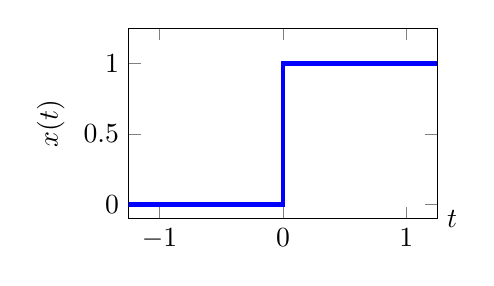
\begin{tikzpicture}
            \begin{axis}[width=5.5cm,height=4cm,ylabel=$x(t)$,xlabel=$t$,ymin=-0.1,ymax=1.25,xmin=-1.25,xmax=1.25,
            xlabel style={at={(1,0)},right,yshift=0pt}]
                \addplot[blue,ultra thick] coordinates {(-2,0) (0,0) (0,1) (2,1)};
                % \addlegendentry{Rectified $\tanh$}
            \end{axis}
        \end{tikzpicture}%
        \caption*{$x(t) &= u(t)$}
  \end{minipage}
    %  \hspace{0.05\textwidth}
      \begin{minipage}[b]{.4\linewidth}
        \begin{tikzpicture}
            \begin{axis}[ width=5.5cm,height=4cm,
            ylabel=$y(t)$,xlabel=$t$,
            % extra x tick style={ticklabel style={fill=white,font=\scriptsize},xticklabel={1}},
            % extra y tick style={ticklabel style={fill=white,font=\scriptsize},yticklabel={1}},
            xlabel style={at={(1,0)},right,yshift=0pt},
            ymin=-0.1,ymax=1.25,yticklabels={1 , , , $\tfrac{1}{a}$},
            xmin=-0.25,xmax=3,xticklabels={ -1, 0, , }]
                \addplot[red,ultra thick] coordinates {(-2,0) (0,0)};
                    \addplot[domain=0:5, red, ultra thick,smooth] {1-e^(-x)} node [pos=0.2, below right,outer sep=1pt,fill=white] {$\tau=\tfrac{1}{a}$};
                % \addlegendentry{$\tau = \frac{1}{a}$}
            \end{axis}
        \end{tikzpicture}%
        \caption*{$y(t) = \tfrac{1}{a}\left(1 - e^{-at}\right)u(t) = \tfrac{1}{p+a}u(t)$}
      \end{minipage}
\end{figure}\\ 
\end{example}
Looking at the two responses of the low-pass filter for inputs of $\delta(t)$ and $u(t)$, what about the graphs tells us that we passed our input signal to a low-pass operator? \smallskip \\
Sudden jumps are things that are high frequencies, and we can see from the graphs that low-pass filters don't allow, or at least attenuate high frequencies, and make the sudden jumps "smoother". By increasing $a$, thereby decreasing the time constant $\tau$ as $\tau = \tfrac{1}{a}$, the system reacts more abruptly, allowing higher frequencies to pass through, and the output resembles the input more.

[What is the time constant?
exponentials go to completion in 5 time constants, a measure to quantize the rate of decay. Time constant has units of time. This phenomenon is obserever everytime the rate of something depends on its value - radio, active decay, Half-life.]

\begin{figure}[H]
    \centering
      \begin{minipage}[b]{.4\linewidth}
        \begin{tikzpicture}
            \begin{axis}[grid=both, width=5.5cm,height=4cm,
            ylabel=$y(t)$,xlabel=$t$,
            % extra x tick style={ticklabel style={fill=white,font=\scriptsize},xticklabel={1}},
            % extra y tick style={ticklabel style={fill=white,font=\scriptsize},yticklabel={1}},
            xlabel style={at={(1,0)},right,yshift=0pt},
            ymin=-0.1,ymax=1.25,yticklabels={1 , , , 1},
            xmin=-0.25,xmax=3,xticklabels={ -1, 0, , }]
                \addplot[red,ultra thick] coordinates {(-2,0) (0,0) (0,1)};
                    \addplot[domain=0:5, red, ultra thick,smooth] {e^(-x/2)} node [pos=0.2, above right,outer sep=1pt,fill=white] {$\tau=2$};
                    \addplot[domain=0:5, blue, ultra thick,smooth] {e^(-5*x)} node [pos=0.2, above right,outer sep=1pt,fill=white] {$\tau=\tfrac{1}{5}$};
                % \addlegendentry{$\tau = \frac{1}{a}$}
            \end{axis}
        \end{tikzpicture}%
        \caption*{$y(t) = e^{-at}u(t) = \tfrac{1}{p+a}\delta(t)$}
  \end{minipage}
    %  \hspace{0.05\textwidth}
      \begin{minipage}[b]{.4\linewidth}
        \begin{tikzpicture}
            \begin{axis}[grid=both, width=5.5cm,height=4cm,
            ylabel=$y(t)$,xlabel=$t$,
            % extra x tick style={ticklabel style={fill=white,font=\scriptsize},xticklabel={1}},
            % extra y tick style={ticklabel style={fill=white,font=\scriptsize},yticklabel={1}},
            xlabel style={at={(1,0)},right,yshift=0pt},
            ymin=-0.1,ymax=1.25,yticklabels={1 , , , $\tfrac{1}{a}$},
            xmin=-0.25,xmax=3,xticklabels={ -1, 0, , }]
                \addplot[red,ultra thick] coordinates {(-2,0) (0,0)};
                    \addplot[domain=0:5, red, ultra thick,smooth] {1-e^(-x/2)} node [pos=0.2, below right,outer sep=1pt,fill=white] {$\tau=2$};
                    \addplot[domain=0:5, blue, ultra thick,smooth] {1-e^(-5*x)} node [pos=0.2, below right,outer sep=0.5pt,fill=white] {$\tau=\tfrac{1}{5}$};
                % \addlegendentry{$\tau = \frac{1}{a}$}
            \end{axis}
        \end{tikzpicture}%
        \caption*{$y(t) = \tfrac{1}{a}\left(1 - e^{-at}\right)u(t) = \tfrac{1}{p+a}u(t)$}
      \end{minipage}
         \caption*{Low-pass operator with time constants $\tau = \tfrac{1}{5}$ and $\tau = 2$}
\end{figure}\\
\textbf{The High-Pass Operator}\\
Referring to the RC circuit that passes low frequencies, can you think of how we could change components to pass high frequencies?\\
\begin{figure}[h]
\centering
\begin{circuitikz}[scale = 1.25]
\draw
    (0,0) to[V, v=$V_s(t)$, invert] (0,1.5)
    to[C, l_=$C$, -*] (2,1.5)
    node[label={above:$n$}] {}
    to[R, l_=$R$, v^=$v(t)$] (2,0)
    -- (1,0) node[ground]{}
    -- (0,0);
\end{circuitikz}
\caption*{RC circuit that passes high frequencies}
\end{figure}\\
Nodal analysis at node $n$ give us
\begin{align*}
    C\dv{v(t) - V_s(t)}{t} + \frac{v(t)}{R} &= 0 \\
    \dv{v}{t} + \frac{v(t)}{\tau} &= \dv{V_s(t)}{t} \\
\intertext{The general form of the differential equation is}
    y' + ay &= x' \\
    \big[p+a\big]y &= px \\
    y &= \frac{1}{p+a}\big[px\big]
\end{align*}
From the notation above, it's clear that we can think of this as applying the Heaviside operator $p$ to the input $x(t)$, and then applying the low-pass operator to the result. Another way to think of $\tfrac{1}{p+a}p$ is that it is a new operator with the symbol $\tfrac{p}{p+a}$ operating on our input. So let's try to figure out what this new operator, the high-pass operator, does to our input. We'll use the low-pass operator to figure this out.\\
Restating the low-pass operator for ease of reference,
\begin{align*}
\hspace{3.0cm} \Aboxed{\frac{1}{p+a}x(t) &=  e^{-at}\frac{1}{p}\Big[e^{at}x(t)\Big] = e^{-at} \int_{-\infty}^{t}e^{a\tau}x(\tau)\dd{\tau}}  \\
    \therefore y &= \frac{p}{p+a}\big[x(t)\big] = \frac{1}{p+a}\big[p\,x(t)\big] \\
    &= e^{-at} \int_{-\infty}^{t} e^{a\tau}px(\tau) \dd{\tau} \\
    &= e^{-at} \int_{-\infty}^{t} e^{a\tau}x'(\tau) \dd{\tau}
\intertext{Integrating by parts with $u = e^{a\tau}$ and $v' = x'(\tau)$,}
    &= e^{-at}\left[e^{at}x(t)- a\int_{-\infty}^{t} e^{a\tau}x(\tau)\dd{\tau} \right] \\
    &= x(t) - a\left[e^{-at}\int_{-\infty}^{t} e^{a\tau}x(\tau)\dd{\tau}\right]
\intertext{The equation in the brackets is exactly our low-pass operator, so}
    y &= x(t) - a\frac{1}{p+a}x(t) \\
      &= \left[1 - a\frac{1}{p+a}\right]x(t)
\intertext{where $1$ is defined as the unity operator. Thus,}
\frac{p}{p+a}\big[x(t)\big] &= \left[1 - a\frac{1}{p+a}\right]x(t)
\intertext{If we treat $p$ as a rational function algebraically, the right hand side is}
                &= \left[1 - \frac{a}{p+a}\right]x(t) \\
                &= \frac{p+a-a}{p+a}\big[x(t)\big] \\
                &= \frac{p}{p+a}\big[x(t)\big]
\end{align*}
We can see from the result above that the Heaviside operator behaves as a rational function algebraically, and so the algebraic properties of association, commutation, and distribution apply to the Heaviside operator, which is motivation behind using the operator to solve differential equations. \textbf{The power of the operator is that it allows us deal with differential equations as rational functions.} This examples illustrates that the Heaviside operator behaves as a rational function algebraically and from now on, we'll treat the operator as a rational function, and no formal proof will be given. (For those who scoff at the lack of rigour, Oliver Heaviside would say to you,\enquote{Shall I refuse my dinner because I do not fully understand the process of digestion?}) \smallskip \\ \\
Now, in general, if we have the operator of the form $\frac{p+a}{p+b}$, then
\begin{align*}
    \frac{p+a}{p+b} &= \frac{p+b-b+a}{p+b} \\
    &= \frac{p+b}{p+b} + \frac{a-b}{p+b} \\
    &= 1 + \frac{a-b}{p+b}
\intertext{So if we want to know the step response of this system, }
    y(t) &= \left[1 + \frac{a-b}{p+b}\right]u(t) \\
        &= u(t) + \frac{a-b}{p+b}u(t)
\end{align*}
\begin{figure}[H]
    \centering
      \begin{minipage}[b]{.4\linewidth}
        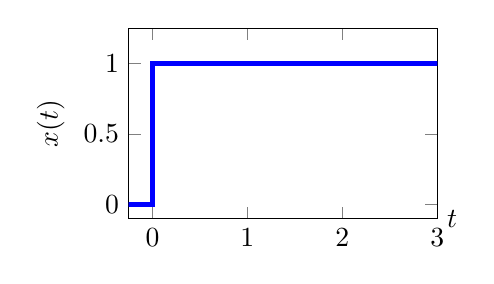
\begin{tikzpicture}
            \begin{axis}[width=5.5cm,height=4cm,ylabel=$x(t)$,xlabel=$t$,ymin=-0.1,ymax=1.25,xmin=-0.25,xmax=3,
            xlabel style={at={(1,0)},right,yshift=0pt}]
                \addplot[blue,ultra thick] coordinates {(-2,0) (0,0) (0,1) (4,1)};
                % \addlegendentry{Rectified $\tanh$}
            \end{axis}
        \end{tikzpicture}%
        \caption*{$x(t) &= u(t)$}
  \end{minipage}
    %  \hspace{0.05\textwidth}
      \begin{minipage}[b]{.4\linewidth}
        \begin{tikzpicture}
            \begin{axis}[ width=5.5cm,height=4cm,
            ylabel=$y(t)$,xlabel=$t$,
            % extra x tick style={ticklabel style={fill=white,font=\scriptsize},xticklabel={1}},
            % extra y tick style={ticklabel style={fill=white,font=\scriptsize},yticklabel={1}},
            xlabel style={at={(1,0)},right,yshift=0pt},
            ymin=-0.1,ymax=1.25,yticklabels={1 , , , $\tfrac{a-b}{b}$},
            xmin=-0.25,xmax=3,xticklabels={ -1, 0, , }]
                \addplot[blue,ultra thick] coordinates {(-2,0) (0,0)};
                    \addplot[domain=0:5, blue, ultra thick,smooth] {1-e^(-x)} node [pos=0.2, below right,outer sep=1pt,fill=white] {$\tau=\tfrac{1}{b}$};
                % \addlegendentry{$\tau = \frac{1}{a}$}
            \end{axis}
        \end{tikzpicture}%
        \caption*{$y(t) = \tfrac{a-b}{b}\left(1 - e^{-bt}\right)u(t) = \tfrac{a-b}{p+b}u(t)$}
     \end{minipage}
     \par\vspace*{\fill}
     \vspace{0.5 cm}
    \begin{tikzpicture}
            \begin{axis}[ width=5.5cm,height=5.5cm,
            ylabel=$y(t)$,xlabel=$t$,
            % extra x tick style={ticklabel style={fill=white,font=\scriptsize},xticklabel={1}},
            % extra y tick style={ticklabel style={fill=white,font=\scriptsize},yticklabel={1}},
            xlabel style={at={(1,0)},right,yshift=0pt},
            ymin=-0.1,ymax=2.25,yticklabels={1 , ,1 , $\tfrac{a}{b}$},
            xmin=-0.25,xmax=3,xticklabels={ -1, 0, , }]
                \addplot[red,ultra thick] coordinates {(-2,0) (0,0) (0,1)};
                    \addplot[domain=0:5, red, ultra thick,smooth] {2-e^(-x)} node [pos=0.2, below right,outer sep=1pt,fill=white] {$\tau=\tfrac{1}{b}$};
                % \addlegendentry{$\tau = \frac{1}{a}$}
            \end{axis}
        \end{tikzpicture}
        \caption*{$y(t) = \tfrac{a-b}{b}\left(1 - e^{-bt}\right)u(t) + u(t) = \left[\tfrac{a-b}{p+b}+1\right]u(t)$}
             \par\vspace*{\fill}
\end{figure}\\ 
Thus, the high-pass operator, and any first order system in general, can be broken down into a unity and low-pass operator. \smallskip \\
\textbf{Solving a Second-Order System}\\
All this is well and good for a first-order system, but how about a second-order system? The general equation of a second order system is of the form
\begin{align*}
    \dv[2]{y}{t} + A\dv{y}{t} + By &= x \text{\quad or,} \\
    y'' + Ay' + By &= x \\
\intertext{$y''$ is $p$ operating on $y$ twice --- $p\Big[p\big[y\big]\Big]$ --- so we can write it as $p^2y$}
    p^2y + Apy + By &= x \\
    \left[p^2 + Ap + B\right]y &= x \\
\intertext{This is a polynomial to the second degree, so we can factor it. Letting $A = a + b$, and $B = ab$,}
    \left[p^2 + (a+b)p + ab\right]y &= x \\
    \left[p^2 + ap + bp + ab\right]y &= x \\
    \left[p(p + a) + b(p + a)\right]y &= x \\
    \left[p + a\right]\left[p + b\right]y &= x \\
\end{align*}
Note that we can even change the order of $\left[p + a\right]$ and $\left[p + b\right]$, and we'll get the same result. 
\begin{align*}
    \therefore y &= \frac{1}{p + a}\frac{1}{p + b}x = \frac{1}{p + b}\frac{1}{p + a}x \\
\end{align*}
\begin{example}
Solve 
\begin{align*}
    y'' + 3y' + 2y &= x \text{\quad where,}\\
        x(t) &= \delta(t)
\intertext{\textbf{Answer.} Using the Heaviside operator,}
    \left[p^2 + 3p + 2\right]y &= \delta(t)\\
    \left[p + 1\right]\left[p + 2\right]y &= \delta(t)\\
    y &= \frac{1}{p + 2}\frac{1}{p + 1}\delta(t) \\
      &= \frac{1}{p + 2} \left[e^{-t} \int_{-\infty}^{t}e^{\tau}\delta(\tau)\dd{\tau}\right] \\
      &= \frac{1}{p + 2} \left[e^{-t} \int_{-\infty}^{t}\cancelto{1}{e^{\tau}}\delta(\tau)\dd{\tau}\right] \\
    &= \frac{1}{p + 2} \left[e^{-t}u(t)\right] \\
    &= e^{-2t} \int_{-\infty}^{t}e^{2\tau}e^{-\tau}u(\tau)\dd{\tau} \\
    &= e^{-2t} \int_{-\infty}^{t}e^{\tau}u(\tau)\dd{\tau} \\
    &= e^{-2t}u(t) \int_{0}^{t}e^{\tau}\dd{\tau} \\
    &= \eval{e^{\tau}}_0^t e^{-2t}u(t) \\
    &= (e^t-1) e^{-2t}u(t) \\
    &= (e^{-t}-e^{-2t})u(t) 
\end{align*}
\label{ex054}
\end{example}
We mentioned previously that the impulse was a gigantic shock to the system that brings about all its characteristic behaviors (i.e. the system's natural frequencies), and we can see that the time constants --- represented by reciprocal of the roots of the characteristic polynomial --- $1$ and $\tfrac{1}{2}$, are present in the exponentials in the response. We will not discuss this more now as we will treat it more formally later. \smallskip \\
Actually, there is an easier way to arrive at the result above. From previous calculations, we know that 
\begin{align*}
    \frac{1}{p + a}\delta(t) &= e^{-at}u(t)
\intertext{So if we're able to simplify $\tfrac{1}{p + 2}\tfrac{1}{p + 1}$ to something of the form $\tfrac{K_1}{p + 2}+\tfrac{K_2}{p + 1}$, we can can get the result of $\tfrac{K_1}{p + 2}\delta(t)$ and $\tfrac{K_2}{p + 1}\delta(t)$ individually, and use superposition to get the final result. We want $K_1$ and $K_2$ such that}
    \frac{1}{p + 2}\frac{1}{p + 1} &= \frac{K_1}{p + 2}+\frac{K_2}{p + 1} \numberthis \label{eq491}
\intertext{Let's try to figure out $K_1$. Multiplying both sides by $(p+2)$,}
            \frac{1}{p + 1} &= K_1 + \frac{K_2(p+2)}{p + 1}
\intertext{Setting $p$ to $-2$,}
    \frac{1}{-2 + 1} &= K_1 + \frac{K_2(-2+2)}{p + 1} \\
    \therefore K_1 &= -1
\intertext{Similarly, we can get $K_2$ by multiplying \cref{eq491} by $(p+1)$ and setting $p$ to $-1$,}
    k_2 &= \frac{1}{p+2} = \frac{1}{-1+2} = 1
\intertext{This process is called Partial Fraction Expansion. Thus, applying an impulse to our system, we get}
    y(t) &= \left[\frac{-1}{p + 2}+\frac{1}{p + 1}\right]\delta(t) \\
        &= -e^{-2t}u(t) + e^{-t}u(t)
\end{align*}
which is the same result as we got before. Let's do another example with the same system, but this time let's hit the system at one of its natural frequencies.\\
\begin{example}
Solve
\begin{align*}
    y'' + 3y' + 2y &= x \text{\quad where,}\\
    x(t) &= e^{-t}u(t)
    \intertext{\textbf{Answer.}}
    y &= \frac{1}{p + 2}\frac{1}{p + 1}e^{-t}u(t) 
\intertext{Now, we know that $e^{-t}u(t) = \tfrac{1}{p+1}\delta(t)$, so substituting that in we get}
    y &= \frac{1}{p + 2}\frac{1}{(p + 1)^2}\delta(t) 
\intertext{Performing partial fraction expansion will give us an equation of the form}
\frac{1}{p + 2}\frac{1}{(p + 1)^2} &= \frac{K_1}{p + 2}+\frac{K_2}{(p + 1)^2}+\frac{K_3}{p + 1}
\intertext{Unfortunately, we don't know the general result of $\tfrac{1}{(p + a)^2}\delta(t)$, so going through the partial fraction expansion and superposition route won't be useful. Nevertheless, we will calculate the result using $\tfrac{1}{p+a}x(t) = e^{-at} \int_{-\infty}^{t}e^{a\tau}x(\tau)\dd{\tau}$.}
    y &= \frac{1}{p + 2}\frac{1}{(p + 1)^2}\delta(t) \numberthis \label{eq516}\\
    \therefore y &= \frac{1}{p + 2}\left[e^{-t} \int_{-\infty}^{t}e^{\tau}e^{-\tau}u(\tau)\dd{\tau}\right] \\
        &= \frac{1}{p + 2}\left[e^{-t} \int_{-\infty}^{t}u(\tau)\dd{\tau}\right] \\
        &= \frac{1}{p + 2}\left[e^{-t}u(t)\int_{0}^{t}\dd{\tau}\right] \\
        &= \frac{1}{p + 2}\left[t\,e^{-t}u(t)\right] \numberthis \label{eq520}
    \intertext{When we hit the system at it's natural frequency, the system gets more excited, loosely speaking, than if we hit it at some other frequency and the result is the natural frequency multiplied by $t$ which grows over time, as opposed to the frequency we hit it at being multiplied by a constant. Continuing,}
        &= e^{-2t} \int_{-\infty}^{t}e^{2\tau}\,\tau\,e^{-\tau}u(\tau)\dd{\tau} \\
        &= e^{-2t} \int_{-\infty}^{t}e^{\tau}\,\tau\,u(\tau)\dd{\tau} \\
        &= e^{-2t} u(t)\int_{0}^{t}e^{\tau}\tau\dd{\tau}
        \intertext{Integrating by parts with $u = \tau$ and $v' = e^\tau$,}
        &= e^{-2t} u(t)\left[\tau e^\tau - \int_{0}^{t} e^\tau\dd{\tau}\right] \\
        &= e^{-2t} u(t)\left[t e^t - \eval{e^\tau}_{0}^t\right] \\
        &= e^{-2t} u(t)\left[t e^t - (e^t - 1) \right]\\ 
        &= e^{-2t} u(t)\left[e^t(t - 1) + 1 \right]\\
        &=  \left[e^{-t}(t - 1) + e^{-2t}\right]u(t)
\end{align*}
\label{ex055}
\end{example}
Thus, even the natural frequency we didn't hit the system at came out, but just not as strongly as the natural frequency that we did hit it at. \\

\textbf{What we've done}\\
In this section, we defined the Heaviside operator, $p$, as the differential with respect to time. We motivated the operator by explaining that all the algebraic properties apply to it, and we saw a glimpse of this when deriving the High-Pass Operator. We further explained that this fact turned solving differential equations into solving algebraic problems. \\
We then saw the consequence of this in solving a second-order system; we treated the operator on $y(t)$ as a function and we were hence able to factorize it, and apply the inverse of the factors to the input. Thus, we fulfilled what we set out to examine in this section which was to WHATTTTTTTTTTT. \smallskip \\
\textbf{Where we're going}\\
We also saw a glimpse of where we're going in \Cref{ex054}; by performing partial fraction expansion on the operator with factors of $p$ in the denominator (i.e. $\tfrac{1}{(p+2)(p+1)}$), we were able to simplify the operator into a sum of simpler operator with irreducible factors of $p$ in the denominator (i.e. $\tfrac{-1}{p+2}\text{+}\tfrac{1}{p+1}$). Thus, if we knew the general result of the simpler operators on our specific input (i.e. $\tfrac{1}{p+a}x(t)$), we could get the result of the simpler operators individually and then by superposition, we could sum the individual responses to get to the final response. \smallskip \\
But this is not that useful; the effect an operator has on one type of input is not generalize-able to another type of input (for example, $\tfrac{1}{p+a}\delta(t)$ is different from $\tfrac{1}{p+a}u(t)$). Hence, for this to be useful we would have to figure out the effect an operator has on every type of input and create a lookup table of some sort. That would be tedious, but in \Cref{ex055} we saw the solution to this problem; we can also convert the input into some operator operating on an impulse $\delta(t)$ (i.e. $x(t) = e^{-t}u(t) = \tfrac{1}{p+1}\delta(t)$). This meant that after multiplying to obtain the system operator and factorizing it (i.e. $\tfrac{1}{p + 2}\tfrac{1}{(p + 1)^2}\delta(t)$), we could use partial fraction expansion to simplify the operator into a sum of simpler operators and then from the general result of each operator acting on $\delta(t)$, we could figure out the specific result! Hence, we simplified the only input we need to consider to the impulse function, $\delta(t)$. \\
But we quickly saw the limitation of this method; we generated an operator of the form $\tfrac{K_2}{(p+a)^2}$ in the partial fraction expansion, and since we didn't know the general result of that operator, the partial fraction expansion and superposition method wasn't so useful. But the good news is that if we did know the result, the response would have been very easy to calculate. \medskip 

But surely we can't do this for every single system; imagine trying to come up with operators to solve 3rd, 4th, 5th order system. In fact, we'll explore this now, but let's define a few terms first. \smallskip \\

\textbf{Definitions}\\
The general form of a system is
\begin{align*}
    {y^{\left( m \right)}\left( t \right)} + {a_{m - 1}}{y^{\left( {m - 1} \right)}\left( t \right)} +  \cdots  + {a_1}y'\left( t \right) + {a_0}y\left( t \right) &= {x^{\left( n \right)}\left( t \right)} + {b_{n - 1}}{x^{\left( {n - 1} \right)}\left( t \right)} +  \cdots  + {b_1}x'\left( t \right) + {b_0}x\left( t \right) \\
    \left[{p^m} + {a_{m - 1}}{p^{m - 1}} +  \cdots  + {a_1}p + {a_0}\right]y(t) &= \left[{p^n} + {b_{n - 1}}{p^{n - 1}} +  \cdots  + {b_1}p + {b_0}\right]x(t)\\
    y(t) &= \frac{{p^n} + {b_{n - 1}}{p^{n - 1}} +  \cdots  + {b_1}p + {b_0}}{{p^m} + {a_{m - 1}}{p^{m - 1}} +  \cdots  + {a_1}p + {a_0}}x(t)
\end{align*}
where $y(t)$ is the output, or system's response, and $x(t)$ is the input. Note that the derivatives of the input present in the above equation is due to the system (as in the case of the circuit used to derived the High-Pass operator), and is not part of what we feed into the system. \\
The above equation can also be represented by the following diagram.
\begin{figure}[H]
    \centering
\begin{tikzpicture}[block/.style={draw, rectangle, minimum height=1cm}]
    \node (box) [block] {$\quad H(p) \quad$}
    node (caption) [below=0.1cm of box] {System}
    node (in1)     [left=1.5cm of box]     {$x(t)$}
    node (out1)    [right=1.5cm of box]    {$y(t)$}
    foreach \X in {1}
    {(in\X) edge[->] (box.west |- in\X)
    (box.east |- out\X) edge[->] (out\X)};
\end{tikzpicture}
\end{figure}
The entire operator that operates on our input, $x(t)$, to produce the system's response, $y(t)$, is called the \textbf{System Operator}. It is denoted by $H(p)$. 
\begin{equation*}
    y(t) = H(p)\,x(t) \numberthis \label{eq571}
\end{equation*}
Now, the impulse response of a system is the response of the system to an impulse.
\begin{align*}
    x(t) &= \delta(t) \\
    h(t) = y(t) &= H(p)\,x(t) \\
    \therefore h(t) &= H(p)\,\delta(t) \numberthis \label{eq577}
\intertext{We'll generalize the notation in \Cref{eq577} to all functions.}
    f(t) &= F(p)\,\delta(t)
\end{align*}
\begin{figure}[H]
    \centering
\begin{tikzpicture}[block/.style={draw, rectangle, minimum height=1cm}]
    \node (box) [block] {$\quad F(p) \quad$}
    node (caption) [below=0.1cm of box] {Function Operator}
    node (in1)     [left=1.5cm of box]     {$\delta(t)$}
    node (out1)    [right=1.5cm of box]    {$f(t)$}
    foreach \X in {1}
    {(in\X) edge[->] (box.west |- in\X)
    (box.east |- out\X) edge[->] (out\X)};
\end{tikzpicture}
\end{figure}
Thus, $F(p)$ is the operator that generates $f(t)$ from an impulse $\delta(t)$. Similarly,
\begin{align*}
    x(t) &= X(p)\,\delta(t) \numberthis \label{eq595} \\
    y(t) &= Y(p)\,\delta(t)\numberthis \label{eq596}
\intertext{where $X(p)$ is known as the \textbf{input operator} and $Y(p)$ is known as the \textbf{output operator}.\\Substituting \Cref{eq595} and \Cref{eq596} into \Cref{eq571},}
    Y(p)\,\delta(t) &= H(p)\,X(p)\,\delta(t) \\
   \iff Y(p) &= H(p)\,X(p)
\end{align*}
To find a system's response, our aim will be to find $H(p)$ (by using the Heaviside operator, $p$, for differentials with respect to time in the equation of a system) and $X(p)$ (by converting our input into the operator that generates our input from an impulse using a catalog), then simplify $Y(p)$ using long division, factorization and partial fraction expansion, and lastly, converting the result of each of the simplified operators acting on $\delta(t)$ back to time-domain functions using a catalog, and summing them up.\smallskip\\
The point of all this is that it makes our systems tractable and understandable. We can see what parts of the system or input contributes what to the response, and can therefore make informed design decisions. But won't our catalog be big? What's the point of this exercise if we have to memorise a big look-up table? Let's go back to exploring this equation.

\textbf{The importance of first and second order systems}

The general form of a system is
\begin{align*}
    {y^{\left( m \right)}\left( t \right)} + {a_{m - 1}}{y^{\left( {m - 1} \right)}\left( t \right)} +  \cdots  + {a_1}y'\left( t \right) + {a_0}y\left( t \right) &= {x^{\left( n \right)}\left( t \right)} + {b_{n - 1}}{x^{\left( {n - 1} \right)}\left( t \right)} +  \cdots  + {b_1}x'\left( t \right) + {b_0}x\left( t \right) \\
    \left[{p^m} + {a_{m - 1}}{p^{m - 1}} +  \cdots  + {a_1}p + {a_0}\right]y(t) &= \left[{p^n} + {b_{n - 1}}{p^{n - 1}} +  \cdots  + {b_1}p + {b_0}\right]x(t)\\
    y(t) &= \frac{{p^n} + {b_{n - 1}}{p^{n - 1}} +  \cdots  + {b_1}p + {b_0}}{{p^m} + {a_{m - 1}}{p^{m - 1}} +  \cdots  + {a_1}p + {a_0}}x(t)
\end{align*}
where $n$ is the order of the numerator and $m$ is the order of the denominator. \\
Case 1: If $n >= m$, we can perform long division and we'll end up 
\begin{align*}
y(t) &= \left[c_{n-m}p^{n-m} + \cdots + c_0p^{0}  + \frac{b_{m - 1}{p^{m-1}} + \cdots  + {b_1}p + {b_0}}{{p^m} + \cdots  + {a_1}p + {a_0}}\right]x(t)
\end{align*}
where $c$ is some natural number. We don't have to worry about the operators of the form $c_ip^i$ as we can apply them directly by differentiating $x(t)\;i$ times and multiplying by $c_i$. We'll treat the proper fraction the same as the next case.\smallskip \\
Case 2: If $n < m$, we have a proper fraction.\\
According to the Fundamental Theorem of Algebra, any $m^{th}$ order polynomial with real coefficients can be factored into first and second order polynomials. The second order polynomials can be further factored into two first order polynomials with complex roots that are conjugates of each other. Thus,
\begin{align*}
    y(t) &= \frac{{p^n} + {b_{n - 1}}{p^{n - 1}} +  \cdots  + {b_1}p + {b_0}}{{p^m} + {a_{m - 1}}{p^{m - 1}} +  \cdots  + {a_1}p + {a_0}}x\left( t \right) \\
     &= \frac{{p^n} + {b_{n - 1}}{p^{n - 1}} +  \cdots  + {b_1}p + {b_0}}{(p-r_m)(p-r_{m-1})\cdots(p-r_1)}x(t)
\end{align*}
where $r_i \in \mathbb{C}$. \\
We can then perform partial fraction expansion, and simplify the system operator into a sum of simpler operators with the operator $p$ to the first or second order in the denominator. \textbf{This means that the response of any $m^{th}$ order system can be broken down into the sum of responses of first and second order system!} This is why the response of first and second order systems are studied in detail; the dynamics of any order system simplify to the dynamics present in first and second order systems. \smallskip \\
\textbf{We'll show that there are, in fact, only four different kinds of simplified operators we can get after partial fraction expansion.} We're building to this look-up table (or catalog) and we'll do so through examples in the following section. \smallskip \\

% All this is very abstract, and was to give the reader an insight of what we're builing to. We're now going develop our catalog by going through examples, and then generalizing our results to add to our catalog. Further, we'll come up a lot of results for our catalog, but we'll show that they simplify to five forms that subsume all the multiple forms we're going to come up with. 





% Convolution - Super important that you understand what's happening here because this is the foundation of figuring out the reponse by a system. Later on we'll abstract on this, but this is very important so learn it

% Lec 11 to 15
% Impulse Response

% Dirac Delta

% Ramp Function

% Getting functions from a diagram of it



% Examples are best seen through videos!

% Simple circuit exmaple LR
% Some other circuit 
% Ossiloscipe low-entropy forms - \textbf{dynamics vs constant}
% \textbf{Impedance and Conductance Operators}
% Nodal Analysis with Heaviside operator (Y Matrix det order is order of the system)

% Complex Numbers e thetha
% Second order system response (we get sum of two first order, multiple root, sin) [how to get multiplicity - is it general mathematical result? ]

% Formal Partial Fraction Expansion
% 2 Examples (System diagram of summation)

% PFE with multiple roots (expanding the multiple roots)
% Equation and then say watch this video for example

% Catalog - Do expanded catalog fully - Example then generalized form??????
% Convolution in Time Domain corresponds to multiplication in operator domain. 
% Good example here

% Time Delay

% Assumption: Lumped Circuit Elements (equation of wavelength), LTI Systems
\section{x. A big a-side: Solving differential equations with the p operator}
\section{x. The Catalog - convert between time and operator domain}
{\renewcommand{\arraystretch}{2.25}
\begin{table}[!htb]
\centering
\begin{tabular}{@{}LL@{}}
\toprule
x(t) = X(p)\delta(t)       & X(p)                                   \\ \midrule
\delta(t)                  & 1                                      \\
u(t)                       & \frac{1}{p}                            \\
r(t) = t \cdot u(t)        & \frac{1}{p^2}                          \\
\frac{t^m}{m!}\,u(t)         & \frac{1}{p^{m+1}}                      \\
e^{-rt}\,u(t)                & \frac{1}{p+r}                          \\
\frac{t^m}{m!}e^{-rt}\,u(t)  & \frac{1}{(p+r)^{m+1}} \\
 \bottomrule
\end{tabular}
\caption*{Our Current Catalog}
\end{table}}
Now that we've listed waveforms and their corresponding heavyside operator that we're familiar with, we will derive the rest of the possible second order rational functions we could get. Instead of listing the operator and figuring out the response to $\delta(t)$, we will start with the waveform and see if we can derive the operator (i.e. the rational function) that could produce it using what we know from the current catalog.

\subsection*{What about $\cos(\wnt)u(t)$?}

Can we use any of the previous operators to figure this out? I'd suggest you try before continuing. \\
From ....., we know that $\cos(\wnt) = \frac{ e^{\jwnt} + e^{-\jwnt}}{2}$.
Thus, 
\begin{align*}
\cos(\wnt)u(t) &= \left[\frac{ e^{\jwnt} + e^{-\jwnt}}{2} \right]u(t) \\ 
 &= \frac{1}{2} \left[ e^{\jwnt} u(t) +  e^{-\jwnt} u(t) \right] \\
 &= \frac{1}{2} \left[\frac{1}{p - \jwn} + \frac{1}{p + \jwn} \right] && \text{(from the catalog)} \\
 &= \frac{1}{2} \left[\frac{p + \jwn + p - \jwn}{p^{2} - (\jwn)^{2}} \right] \\
 &= \frac{1}{2} \left[\frac{2p}{p^{2} + \wn^{2}} \right] \\
 &=  \frac{p}{p^{2} + \wn^{2}}
\end{align*}

\subsection*{What about $\sin(\wnt)u(t)$?}

If you had to guess, what do you think it could be? \\
We know that $\sin(\wnt) = \frac{ e^{\jwnt} - e^{-\jwnt}}{2j}$.
Thus, 
\begin{align*}
\sin(\wnt)u(t) &= \left[\frac{ e^{\jwnt} - e^{-\jwnt}}{2j} \right]u(t) \\
&= \frac{1}{2j} \left[ e^{\jwnt} u(t) -  e^{-\jwnt} u(t) \right] \\
&= \frac{1}{2j} \left[\frac{1}{p - \jwn} - \frac{1}{p + \jwn} \right] && \text{(from the catalog)} \\
&= \frac{1}{2j} \left[\frac{p + \jwn - p + \jwn}{p^{2} - (\jwn)^{2}} \right] \\
&= \frac{1}{2j} \left[\frac{2\jwn}{p^{2} + \wn^{2}} \right] \\
&=  \frac{\wn}{p^{2} + \wn^{2}}
\intertext{
\subsection*{What about $e^{-\sigma t}\cos(\wnt)u(t)$?}
If you had to guess, what do you think it could be? (your guess should reduce to the operator for $\cos(\wnt)u(t)$ for $\sigma = 0$, and to $e^{-\sigma t}$ for $\wn = 0$)
}
        e^{-\sigma t}\cos(\wnt)u(t) &= e^{-\sigma t}\left[\frac{ e^{\jwnt} + e^{-\jwnt}}{2} \right] u(t) \\
        &= \frac{1}{2} \left[ e^{(\jwn - \sigma)t} + e^{(-\jwn - \sigma)t} \right] u(t) \\
        &= \frac{1}{2} \left[ \frac{1}{p + (\sigma - \jwn)} + \frac{1}{p + (\sigma + \jwn)} \right] u(t) && \text{(from the catalog)} \\
        &= \frac{1}{2} \left[ \frac{2p + 2\sigma}{(p + \sigma + \jwn)(p + \sigma - \jwn)} \right] u(t) \\
        &= \frac{p + \sigma}{(p + \sigma)^{2} + \wn^{2}}
\intertext{
\subsection*{What about $e^{-\sigma t}\sin(\wnt)u(t)$?}
Extrapolating from $\cos(\wnt)u(t)$ and $\sin(\wnt)u(t)$, a good guess could be $\frac{\wn}{(p + \sigma)^{2} + \wn^{2}}$. Let's see what it really is.
}
        e^{-\sigma t}\sin(\wnt)u(t) &= e^{-\sigma t}\left[\frac{ e^{\jwnt} - e^{-\jwnt}}{2j} \right] u(t) \\
        &= \frac{1}{2j} \left[ e^{(\jwn - \sigma)t} - e^{(-\jwn - \sigma)t} \right] u(t) \\
        &= \frac{1}{2j} \left[ \frac{1}{p + (\sigma - \jwn)} - \frac{1}{p + (\sigma + \jwn)} \right] u(t) && \text{(from the catalog)} \\
        &= \frac{1}{2j} \left[ \frac{2\jwn}{(p + \sigma + \jwn)(p + \sigma - \jwn)} \right] u(t) \\
        &= \frac{\wn}{(p + \sigma)^{2} + \wn^{2}}
\end{align*}

% [Side note: $\sigma$ vs $r$ notation
% When we write a pair of complex conjugate numbers, we often show them as $\sigma \pm \jwn$ which implies that $\sigma$ and $\jwn$ are real numbers. This has become convention, and thus $\sigma$ implies a real number, but $r$ implies any number which includes complex numbers. 

% In the above example, we use $\sigma$ instead of $r$ purposely. $e^{-r t}\cos(\wnt)u(t)$ implies we're generating a complex waveform in the time domain which is not possible. For example, what would $(1 + 2j)u(t)$ look like? In our notion of things this does not make sense. 

% You may ask, what about $e^{-rt}u(t)$? Isn't that a complex waveform in the time domain?]

\subsection*{The Final Catalog}
{\renewcommand{\arraystretch}{2.25}
\begin{table}[!htb]
\begin{minipage}[b]{.5\linewidth}
\centering
\begin{tabular}{@{}LL@{}}
\toprule
x(t) = X(p)\delta(t)       & X(p)                                   \\ \midrule
\delta(t)                  & 1                                      \\
u(t)                       & \frac{1}{p}                            \\
r(t) = t \cdot u(t)        & \frac{1}{p^2}                          \\
\frac{t^m}{m!}\,u(t)         & \frac{1}{p^{m+1}}                      \\
e^{-rt}\,u(t)                & \frac{1}{p+r} 
\\
\frac{t^m}{m!}e^{-rt}\,u(t)  & \frac{1}{(p+r)^{m+1}} \\
\cos(\wnt)\,u(t)              & \frac{p}{p^2 + \wn^2}                   \\
\sin(\wnt)\,u(t)              & \frac{\wn}{p^2 + \wn^2}                  \\
e^{-\sigma t}\cos(\wnt)\,u(t) & \frac{p + \sigma}{(p+\sigma)^2 + \wn^2} \\
e^{-\sigma t}\sin(\wnt)\,u(t) & \frac{\wn}{(p+\sigma)^2 + \wn^2}         \\ \bottomrule
\end{tabular}
\caption*{Final Catalog}
\end{minipage}\hfill%
\begin{minipage}[b]{.5\linewidth}
\centering
\begin{tabular}{@{}LL@{}}
\toprule
x(t) = X(p)\delta(t)       & X(p)                                   \\ \midrule
\delta(t)                  & 1                                      \\
\frac{t^m}{m!}\,u(t)         & \frac{1}{p^{m+1}}                      \\
\frac{t^m}{m!}e^{-rt}\,u(t)  & \frac{1}{(p+r)^{m+1}} \\
\cos(\wnt)\,u(t)              & \frac{p}{p^2 + \wn^2}                   \\
\sin(\wnt)\,u(t)              & \frac{\wn}{p^2 + \wn^2}                  \\
e^{-\sigma t}\cos(\wnt)\,u(t) & \frac{p + \sigma}{(p+\sigma)^2 + \wn^2} \\
e^{-\sigma t}\sin(\wnt)\,u(t) & \frac{\wn}{(p+\sigma)^2 + \wn^2}         \\ \bottomrule
\end{tabular}
\caption*{Simplified Final Catalog}
\end{minipage}
\end{table}}
What is special about this table? According to the fundamnetal theorem of algebra, we can factor any $n^{th}$ order polynomial into first and second order polynomials with real coefficients. This table contains all the first and second order polynomials you can get from the partial fraction expansion of rational functions! \\
Thus, these waveforms are the only sort of waveforms that we can get out of a system that can be described with rational functions, which is all circuits with lumped circuit elements. There are other systems that are not lumped whose responses do not look like this, but if it is lumped and if we're dealing with circuit elements of a linear kind, these are the responses. 

\textbf{Example to motivate the usefulness of the catalog:} \\
Suppose we would like to solve the differential equation
\begin{align*}
    y'' + 3y' + 2y &= x(t)
\intertext{where the input is} x(t) &= 4 \cos(t) u(t)
\intertext{Now, combining the above two equations and converting to operator domain using the catalog,}
    \left[p^2 + 3p + 2\right]y &= \frac{4p}{p^2 + 1}\delta(t)
\intertext{Factoring and rearranging for y(t),}
y(t) &= \frac{4p}{(p + 1)(p + 2)(p^2 + 1)}\delta(t)
\end{align*}

\begin{align*}
    Y(p) &= \frac{4p}{(p + 1)(p + 2)(p^2 + 1)} \\
        &= \frac{-2}{p+1} + \frac{8}{5}\left(\frac{1}{p+2}\right) + \frac{1}{5}\left(\frac{1+3j}{p+j}\right) + \frac{1}{5}\left(\frac{1-3j}{p-j}\right) \\
        &= \frac{-2}{p+1} + \frac{8}{5}\left(\frac{1}{p+2}\right) + \frac{2}{5}\left(\frac{p+3}{p^2 + 1}\right) \\
        &= \frac{-2}{p+1} + \frac{8}{5}\left(\frac{1}{p+2}\right) + \frac{2}{5}\left(\frac{p}{p^2 + 1}\right)
        + \frac{2}{5}\left(\frac{3}{p^2 + 1}\right) \\
\intertext{(the partial fraction expansion working out can be seen \href{https://youtu.be/D8w2qZKb5Ug?t=2355}{here})\\
    Using the catalog to convert to time domain,}
    y(t) &= \left(-2e^{-t} + \frac{8}{5} e^{-2t} + \frac{2}{5} \cos(t) + \frac{6}{5} \sin(t)\right)u(t)
\end{align*}

\textbf{Putting it all together} \\
The catalog is extremely useful because it allows us to get the response of a system to any input using partial fraction expansion, multiplication, and the catalog. There's no need for any integration or convolution!

Summary of the method:
\begin{enumerate}
    \item Get the differential equation of the system in terms of the p operator.
    \item Convert input from time domain to operator domain using catalog (i.e. Find $X(p)$ where $x(t) = X(p)\delta(t)$).
    \item Rearrange to get $y(t)$ on one side such that $y(t) = Y(p)\,\delta(t)$, and simplify $Y(p)$ using partial fraction expansion.
    \item Convert $Y(p)\,\delta(t)$ to time domain using the catalog.
\end{enumerate}

\textbf{Concluding Notes} \\
We have now developed a powerful method that not only allows you to do the calculations in certain ways that avoid integration or convolution, which make it easier to do by hand, but also this method gives us additional insight when it comes to design which helps us choosing elements to get the output we desire. 

\textbf{Example to motivate how the operator domain helps with design} \\
\begin{figure}[h]
    \centering
    \begin{tikzpicture}[
    scale=0.5,
        %Environment Config
        MyArrow/.style={%Style for the current
            -Stealth,
            blue,
            line width=1.5pt,
            shorten >= 5pt,
            shorten <= 1pt
        },
        Vref/.style={%Style for the voltage reference
            draw=none,
            postaction={decorate,decoration={markings,mark=at position 0.5 with {\node[anchor=east]{\Large #1};}}},
            postaction={decorate,decoration={markings,mark=at position 0.20 with {\node{$\bm{+}$};}}},
            postaction={decorate,decoration={markings,mark=at position 0.80 with {\node{ $\bm{-}$};}}}
        },
        Numbered/.style = {% Style for circle marks
                draw,
                circle,
                line width=1.5pt,
                align=center,
                inner sep=4pt,
                label distance=15pt
           }
    ]
    \def\MyOpamp(#1)#2{%Customized opamp
    \begin{scope}[shift={(#1)}]
    %Component Shape
    \draw[line width = 1pt, line join=round] (0,0)++(-1,1.5)
        --++(2.5,-1.5) -- ++(-2.5,-1.5)-- cycle; 
    % Label and component identifier.
    \draw(0,0) node{}; % IC LABEL
    % Draw the pins
    % Some that you have to learn about label nodes, draw lines, and name coordinates in Tikz
    \draw[line width = 1pt] (-1,0.6) node [anchor=180]{\small$-$} -- ++(-0.5,0)  coordinate (#2 IN-); % IN - 
    \draw[line width = 1pt] (-1,-0.6) node [anchor=180]{\small$+$}  -- ++(-0.5,0) coordinate (#2 IN+); % IN +
    \draw[line width = 1pt] (1.5,0)  -- ++(0.5,0) coordinate (#2 OUT); % OUT  
    \end{scope}
    }
    \def\MyGround(#1)#2{%customized ground
    \begin{scope}[shift={(#1)}]
    %Component Shape
    \draw[line width = 0.75pt, line cap=round]
    (0,0) coordinate (#2 GND)++(-0.3,0)--++(0.6,0)
    (0,-0.15)++(-0.2,0)--++(0.4,0)
    (0,-0.29)++(-0.1,0)--++(0.2,0);  
    \end{scope}
    }

    %Put the customzed opamp in position
    \MyOpamp(0,0){1}

    %Put some short nodes
    \draw(-7,0.6) node[ocirc,scale=1.5,line width=1pt](N3){};
    \draw(-3,0.6) node[circ,scale=1.5,line width=1pt](N2){};
    \draw(3,0) node[circ,scale=1.5,line width=1pt](N6){};
    \draw(5.5,0) node[ocirc,scale=1.5,line width=1pt](N6-OUT){};
    \MyGround(-7,-3){1}
    \MyGround(1 GND -| N2){2}
    \MyGround(1 GND -| N6-OUT){3}

    %Draw the Wires and pasive components
    \draw[line width=1pt]
    (N3)%From node N3
        --++(0.1,0)
        to [generic,l=\Large$Z_1$] (N2)
        --(1 IN-)
    (N2)
        --++(0,2) coordinate (N5)
        --++(2.5,0)
        to[generic,l=\Large$Z_2$]++(3,0)
        -| (N6)
    (1 OUT) 
        -- (N6-OUT)
    (1 IN+)
        -|(2 GND);
    %Voltage references
    \draw[Vref=\Large$v_{in}$]
    (N3) 
        -- (1 GND);

    \draw[Vref,color=black]
    (N6-OUT) 
        -- (3 GND) 
        node [midway,
            anchor=west]
            {\Large$\bm{v_{out}} = -\cfrac{Z_2}{Z_1}\;v_{in}$};
    \draw[black]
    (C1 -| 3 GND)
        node [
            inner sep=10pt,
            anchor=west,
        ]{};
        % {\Large$\bm{v_{out}} = -\cfrac{Z_2}{Z_1}\;v_{in}$};

    \end{tikzpicture}
\end{figure}

Suppose we have an op-amp in this configuration. The square boxes represent the impedance of elements that we have to choose. We know that since this is an op-amp with negative feedback, 
\begin{equation}
\label{eqn:op-amp}
    V_{out} = -\frac{Z_2}{Z_1} V_{in}
\end{equation}
Now, suppose we want to build an integrator. What components should we choose for elements 1 and 2? Well, we know that the $\tfrac{1}{p}$ operator is integration. So we have to choose $Z_2$ and $Z_1$ such that we have $p$ in the denominator of \cref{eqn:op-amp}. If $Z_2$ is a capacitor, this fulfills our criteria (making $Z_1$ an inductor also fulfills our criteria, but inductors are generally avoided where possible due to their interference from their magnetic fields, large series resistance and stray capacitance). Since we don't want any other p operators, $Z_1$ must be a resistor. This is in fact how integrators are built.\smallskip \\
Similarly, what if we wanted to differentiate the input voltage with the same circuit setup as above? We know that the p operator is differentiation so we must have p in the numerator of \cref{eqn:op-amp}. Avoiding inductors, $Z_1$ must be a capacitor and since we don't want any other operators, $Z_2$ must be a resistor.


\section{x. Delays and Time Shifts - The last piece of the puzzle}

Suppose we have a system whose impulse response and input are respectively

\begin{figure}[h]
    \centering
      \begin{minipage}[b]{.4\linewidth}
            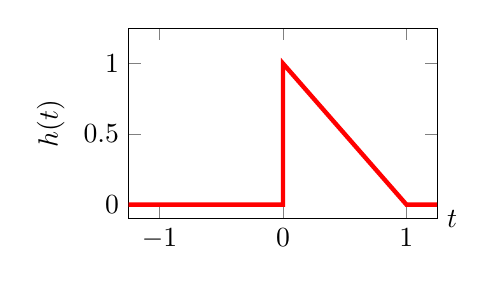
\begin{tikzpicture}
            \begin{axis}[width=5.5cm,height=4cm,ylabel=$h(t)$,xlabel=$t$,ymin=-0.1,ymax=1.25,xmin=-1.25,xmax=1.25,
            xlabel style={at={(1,0)},right,yshift=0pt}]
                % \addlegendimage{ultra thick,red}
                % \addplot[ultra thick,red,mark=*,mark options={fill=white},samples at={-1.1,0}] {0};
                \addplot[red,ultra thick] coordinates {(-2,0) (0,0) (0,1) (1,0) (2,0)};
                % \addplot[ultra thick,blue,mark=*,samples at={0,1.1}] {0.5};
                % \addlegendentry{impulse response}
            \end{axis}
        \end{tikzpicture}%
        \caption*{$h(t) &= u(t) - t\cdot u(t) + (t-1) \cdot u(t-1)$}
  \end{minipage}
    %  \hspace{0.05\textwidth}
      \begin{minipage}[b]{.4\linewidth}
        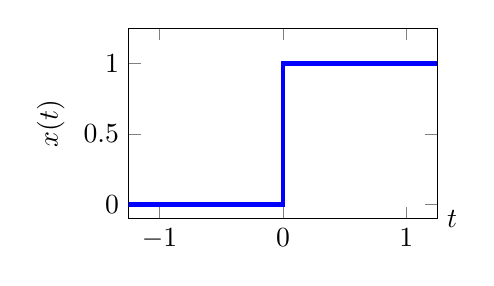
\begin{tikzpicture}
            \begin{axis}[width=5.5cm,height=4cm,ylabel=$x(t)$,xlabel=$t$,ymin=-0.1,ymax=1.25,xmin=-1.25,xmax=1.25,
            xlabel style={at={(1,0)},right,yshift=0pt}]
                \addplot[blue,ultra thick] coordinates {(-2,0) (0,0) (0,1) (2,1)};
                % \addlegendentry{Rectified $\tanh$}
            \end{axis}
        \end{tikzpicture}%
        \caption*{$x(t) &= u(t)$}
      \end{minipage}
\end{figure}%
Now, converting the input to the operator domain, we get
\begin{align*}
    X(p) &= \frac{1}{p}
\intertext{and converting it's impulse response to the operator domain, we get}
H(p) &= \frac{1}{p} - \frac{1}{p^{2}} + \textbf{?}
\intertext{
How do we represent the delay in the operator domain? The operator $\frac{1}{p^{2}}$ is obviously incorrect, so what could it be? 
Let's try to figure this out by looking at the definition of the impulse response}
    h(t) &= H(p) \delta(t)
\end{align*}
From this definition, can we figure out what is $h(t - \tau)$? \\
Let's try to use the Taylor Series Expansion to figure this out.
 \begin{align*}
 h(t - \tau) &= \sum_{k=0}^\infty \frac{(-\tau)^{k}}{k!}h^{k}(t) \\
 &= h(t) - \frac{\tau}{1!} h'(t) + \frac{\tau^{2}}{2!} h''(t) - \frac{\tau^{3}}{3!}h'''(t)+\dotsb 
\intertext{
Since the p-operator is the derivative, $h'(t) = p [h(t)]= p\,H(p)\delta(t)$. In general, $h^{k}(t) = p^{k}\,H(p)\delta(t)$. Thus,}
    h(t - \tau) &= H(p)\delta(t) - \tau pH(p)\delta(t) + \frac{(\tau p)^{2}}{2!} H(p)\delta(t) - \frac{(\tau p)^{3}}{3!} H(p)\delta(t) + \dotsb \\
&= \left[1 - \tau p + \frac{(\tau p)^{2}}{2!} - \frac{(\tau p)^{3}}{3!} + \dotsb \right] H(p)\delta(t) \\
&= e^{-\tau p} H(p) \delta(t)
\intertext{
In general, we have,}
f(t-\tau) &= e^{-\tau p} F(p) \delta(t)
\intertext{But we generally work with $f(t-\tau)u(t-\tau)$ }
\intertext{
Going back to our example above,}
h(t) &= u(t) - t \cdot u(t) + (t-1) \cdot u(t-1) \\
\therefore H(p) &= \frac{1}{p} - \frac{1}{p^{2}} +  e^{-p}\frac{1}{p^2} \intertext{
 Now,}
     y(t) &= H(p) X(p) = \frac{1}{p^2} - \frac{1}{p^{3}} +  e^{-p}\frac{1}{p^3}
\intertext{Using the catalog to convert back to waveforms,}
 y(t) &= t\cdot u(t) - \frac{t^2}{2}u(t) + \frac{(t-1)^2}{2}u(t-1)
\end{align*}

Thus, the complete catalog for systems with lumped elements, and hence rational system operators is


% SHOULD EXPLAIN $e^{-at}x(t) = X(p+a)$

% CATALOG FOR BASE FUNCTIONS AND CATALOG FOR TIME?
% {\renewcommand{\arraystretch}{2.25}
% \begin{table}[!htb]
% \begin{minipage}[b]{.5\linewidth}
% \centering
% \begin{tabular}{@{}LL@{}}
% \toprule
% x(t) = X(p)\delta(t)       & X(p)                                   \\ \midrule
% \delta(t)                  & 1                                      \\
% u(t)                       & \frac{1}{p}                            \\
% r(t) = t \cdot u(t)        & \frac{1}{p^2}                          \\
% \frac{t^m}{m!}\,u(t)         & \frac{1}{p^{m+1}}                      \\
% e^{-rt}\,u(t)                & \frac{1}{p+r} 
% \\
% \frac{t^m}{m!}e^{-rt}\,u(t)  & \frac{1}{(p+r)^{m+1}} \\
% \cos(\wnt)\,u(t)              & \frac{p}{p^2 + \wn^2}                   \\
% \sin(\wnt)\,u(t)              & \frac{\wn}{p^2 + \wn^2}                  \\
% e^{-\sigma t}\cos(\wnt)\,u(t) & \frac{p + \sigma}{(p+\sigma)^2 + \wn^2} \\
% e^{-\sigma t}\sin(\wnt)\,u(t) & \frac{\wn}{(p+\sigma)^2 + \wn^2}         \\
% x(t-\tau)u(t-\tau)    & e^{-\tau p} X(p) \\
% e^{\tau t}x(t)    & X(p + \tau) \\

% \bottomrule
% \end{tabular}
% \caption*{Final Catalog}
% \end{minipage}\hfill%
% \begin{minipage}[b]{.5\linewidth}
% \centering
% \begin{tabular}{@{}LL@{}}
% \toprule
% x(t) = X(p)\delta(t)       & X(p)                                   \\ \midrule
% \delta(t)                  & 1                                      \\
% \frac{t^m}{m!}e^{-rt}\,u(t)  & \frac{1}{(p+r)^{m+1}} \\
% e^{-\sigma t}\cos(\wnt)\,u(t) & \frac{p + \sigma}{(p+\sigma)^2 + \wn^2} \\
% e^{-\sigma t}\sin(\wnt)\,u(t) & \frac{\wn}{(p+\sigma)^2 + \wn^2}         \\
% x(t-\tau)    & e^{-\tau p} X(p) \\
% \bottomrule
% \end{tabular}
% \caption*{Simplified Final Catalog}
% \end{minipage}
% \end{table}}
\end{document}
